\section{Isotropic\_Sqw: A general $S(q,\omega)$ coherent and incoherent scatterer}
\label{s:isotropic-sqw}
\index{Samples!Coherent and incoherent isotropic scatterer}
\index{Coherent and incoherent isotropic scatterer}
\index{Inelastic scattering}

\component{Isotropic\_Sqw}{V. Hugouvieux, E. Farhi}{Sqw$\_{coh}$, $\sigma_{coh}$, Sqw$\_{inc}$, $\sigma_{inc}, V_\rho, \sigma_{abs}, T$}{$q_{min}, q_{max}, \omega_{min}, \omega_{max}, d\phi$, order}{not fully validated}

\begin{figure}
  \begin{center}
    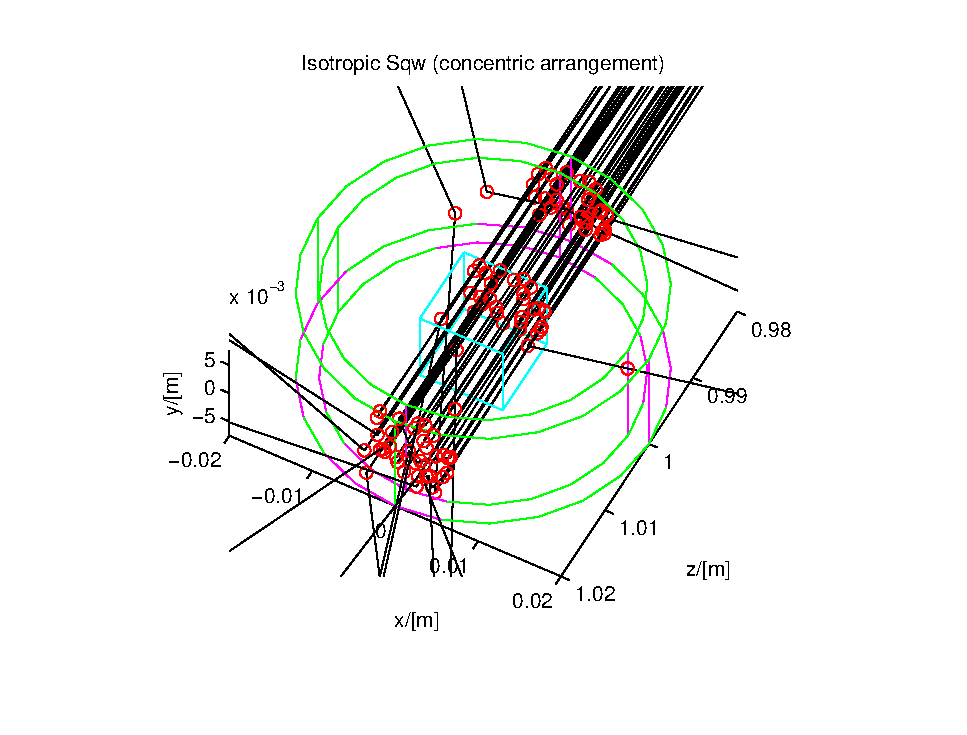
\includegraphics[width=0.9\textwidth]{figures/sqw.eps}
  \end{center}
\caption{An $l-^4$He sample in a cryostat, simulated with the Isotropic\_Sqw component in concentric geometry.}
\label{f:isotropic-sqw}
\end{figure}

This component implements a very gener

\subsection{The theory}

The component assumes that the sample has the structure of a liquid. This stands for indeed normal liquids, glasses (amorphous systems), polymers, and may be extended to powders.

In the case of a homogeneous and classical liquid, the {\it van Hove correlation function}, which describes the time and space correlations in the liquid, can be written:
\begin{equation} \label{eq:vanhove}
G(\vec{r},\tau) = \frac{1}{N} \sum_{i=1}^N \sum_{j=1}^N  \langle\delta[\vec{r} + \vec{r}_i(0) - \vec{r}_j(\tau)]\rangle
\end{equation}
The dynamical structure factor $S(q,\omega)$ is the double Fourier-transform in space and time of the van Hove correlation function $G(r,t)$.

Following Squires (\cite{squires}, p63), the neutron scattered signal for both coherent and incoherent processes is
\begin{equation}
\frac{d^2\sigma}{d\Omega dE_f} = \frac{\sigma}{4\pi}\frac{k_f}{k_i} N S(q, \omega)
\end{equation}
with usual notations. The unit of the dynamical structure factor $S$ is an inverse energy.

\subsection{How does a neutron interact with the material ?}

\subsection{The implementation}